\documentclass[tikz]{standalone}
\usetikzlibrary{calc,arrows}
\usepackage{frenchmath}

\begin{document}
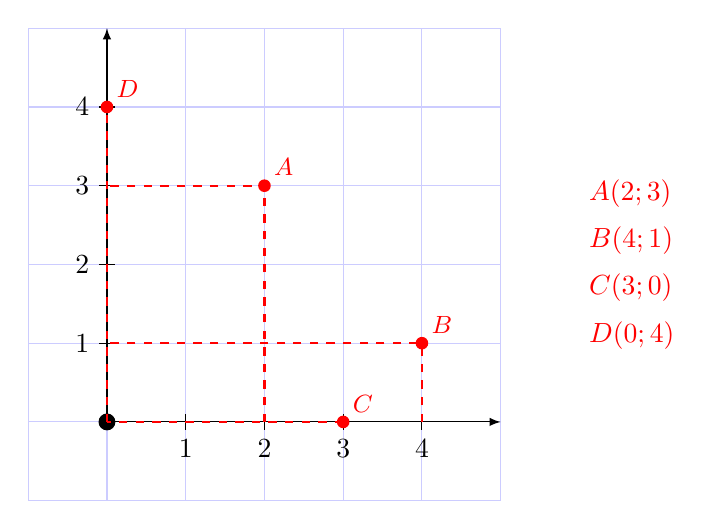
\begin{tikzpicture}
    \draw[color=blue!20!white] (-1,-1) grid (5,5); 
    \draw[fill] (0,0) circle (0.1);
    \draw[-latex] (0,0) -- (5,0);
    \draw[-latex] (0,0) -- (0,5);
    \foreach \n in {1,...,4} {
        \draw (\n,-0.1) node[below] {$\n$} -- (\n,0.1);
    }
    \foreach \n in {1,...,4} {
        \draw (-0.1,\n) node[left] {$\n$} -- (0.1,\n);
    }
    \foreach[count=\i] \p/\x/\y in {A/2/3, B/4/1, C/3/0, D/0/4} {
        \draw[red, dashed, thick] (\x,0) -- (\x,\y) -- (0,\y);
        \fill[red] (\x,\y) circle (0.08);
        \node[font=\small,above right,red] at (\x,\y) {$\p$};
        \node[anchor=west,red] at (6,{3.5-0.6*\i}) {$\p(\x;\y)$};
    }
\end{tikzpicture}
\end{document}